\begin{frame}{Premise of the Paper}
  %% what is the paper trying to solve
\end{frame}

%%%%%%%%%%%%%%%%%%%%%%%%%%%%%%%%%%%%%%%%%%%%%%%%%%
\begin{frame}{Partition Function Woes}
  %% what is the paper trying to solve
\end{frame}

%%%%%%%%%%%%%%%%%%%%%%%%%%%%%%%%%%%%%%%%%%%%%%%%%%
\begin{frame}{Gumbel Distribution}
  \begin{itemize}
  \item Strong Convexity
  %% \item Sub-differential (sub-gradient)
  \item Convex Conjugate
  \item Dual Norm
  \item Strong Smoothness
  \end{itemize}
\end{frame}

%%%%%%%%%%%%%%%%%%%%%%%%%%%%%%%%%%%%%%%%%%%%%%%%%%
\begin{frame}{Gumbel-Max Trick}
  
\end{frame}

%%%%%%%%%%%%%%%%%%%%%%%%%%%%%%%%%%%%%%%%%%%%%%%%%%
\begin{frame}{Gumbel Process}
  %% just put image
\end{frame}

%%%%%%%%%%%%%%%%%%%%%%%%%%%%%%%%%%%%%%%%%%%%%%%%%%
\begin{frame}{Top-Down Construction}
  \begin{figure}
    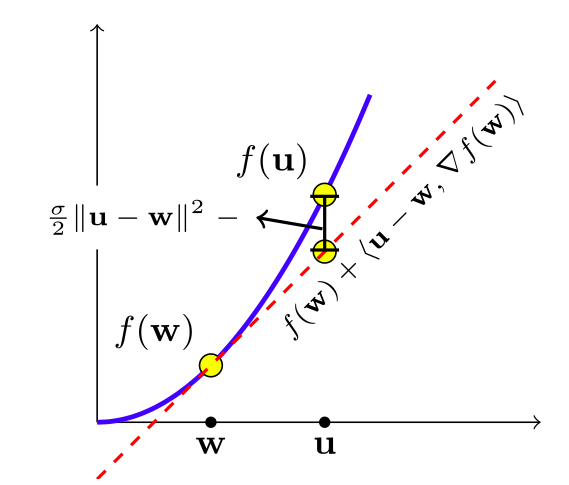
\includegraphics[scale=0.27]{images/str_convex.png}
    \caption{From \cite{ShSh2012}. A $\sigma$ strongly convex function.}
  \end{figure}
\end{frame}
